\documentclass[12pt]{article}
\usepackage[a4paper, margin=1in]{geometry}
\usepackage[protrusion=true, expansion=true]{microtype}
\usepackage[english]{babel}
\usepackage[T1]{fontenc}
\usepackage{amsmath, amsfonts, amssymb, indentfirst, hyperref, float, titlesec, fancyhdr, graphicx, enumitem, tabularx, xcolor}
\usepackage[outputdir=pdf]{minted}

% hyperref setup
\hypersetup{
    colorlinks=true,
    linktoc=all,
    linkcolor=black,
}

\definecolor{codeBackground}{rgb}{0.95, 0.95, 0.97}
\setminted{
  autogobble=true,
  linenos=true,
  breaklines=true,
  bgcolor=codeBackground,
  frame=single,
}

% Paragraph formatting
\setlength{\parindent}{1em}
\setlength{\parskip}{0.5em}

\newcommand\projectTitle{Controller Design}
\newcommand\courseID{AE 308}
\newcommand\studentName{Krith Sanvith Manthripragada}
\newcommand\studentRollNo{180010030}

%------------------------------
% HEADER & FOOTER
%------------------------------
\pagestyle{fancy}
\fancyhf{}% Clear header and footer
\fancyhead[RO]{\studentRollNo}
\fancyhead[L]{\courseID}
\renewcommand{\headrulewidth}{0pt}
\renewcommand{\footrulewidth}{0pt}


% Front Page Definition
\title{ 
  {\Large \textbf{\MakeUppercase{\projectTitle{}}}} \\
  {\large Course Project - \courseID} \vspace{-1em}
}
\author{
  {\large \studentName} \\
  {\large \studentRollNo}
}
\date{}

% Always have this just before \begin{document}
\usepackage{subfiles}

\begin{document}

\maketitle
\thispagestyle{fancy}

\subsection*{Problem Formulation:}
The given transfer is
\begin{equation}
  G(S) = \frac{S+500}{S(S+0.0325)(S^2 + 2.57S + 6667)}
\end{equation}

Given conditions:
\begin{center}
  \(K_V = \text{Ramp Error Constant} = 100 \) \\
  \text{Phase Margin} > \(35^\circ \)
\end{center}

Now, using these above conditions, we need to design a controller using Root Locus Method and we need to determine Resonant Frequency, Resonant Peak and Bandwidth of the Compensated System. Also determine the Transient Response of the System.

\subsection*{Theory:}
Lets look how different types of controllers impact the closed loop behaviour of a given system.
\begin{enumerate}[label={\alph*)}]
  \item \textbf{P Controller:}
  \begin{enumerate}[label={(\roman*)}]
    \item Modifies overall loop gain and hence steady state behaviour.
    
    \item Change dominant pole location and thereby relative and transient response.
  \end{enumerate}

  \item \textbf{PD Controller:}
  \begin{enumerate}[label={(\roman*)}]
    \item It can reduce the overshoot of a proportional controller because PD controller takes into account the rate of change in error.
    
    \item It can improve system tolerances to external disturbances.
  \end{enumerate}

  \item \textbf{PI Controller:}
  \begin{enumerate}[label={(\roman*)}]
    \item It is mainly used for tracking of step and ramp inputs.
    \item Eliminates steady state error.
  \end{enumerate}


  \item \textbf{PID Controller:}
  \begin{enumerate}[label={(\roman*)}]
    \item It can reduce overshoot of system.
    \item Improve system tolerances to external disturbances.
    \item Steady state error decreases.
  \end{enumerate}

  \item \textbf{Lead and Lag Compensator:}
  \begin{enumerate}[label={(\roman*)}]
    \item A Lead Compensator can increase the stability or speed of response of a system.
	  \item A Lag Compensator can reduce the steady state error.
  \end{enumerate}
\end{enumerate}

\subsection*{Design Strategy:}
Let us first understand the system given to us observing the step response of the uncompensated system. \par

\begin{minipage}{0.45\linewidth}
  \begin{figure}[H]
    \centering
    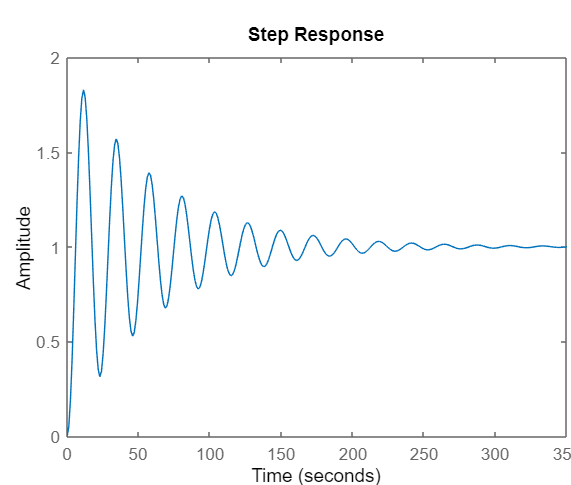
\includegraphics[width=\linewidth]{images/plot1.png}
    \label{fig:plot_1}
  \end{figure}
\end{minipage}%
\hfill
\begin{minipage}{0.45\linewidth}
  \begin{figure}[H]
    \centering
    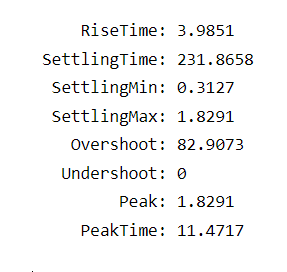
\includegraphics[width=\linewidth]{images/plot2.png}
    \label{fig:plot_2}
  \end{figure}
\end{minipage}

The uncompensated closed loop response has a settling time of \(231.689\) seconds and O.S of 82.7\% which are very large and also has a \(k_v\) of \(2.3\) which is very little compared to our requirement and hence we need to add quite a bit of gain to the system.\par

\begin{minipage}{0.3\linewidth} \par
  Also let us look at the bode plot of the given plant system.
\end{minipage}%
\hfill
\begin{minipage}{0.65\linewidth}
  \begin{figure}[H]
    \centering
    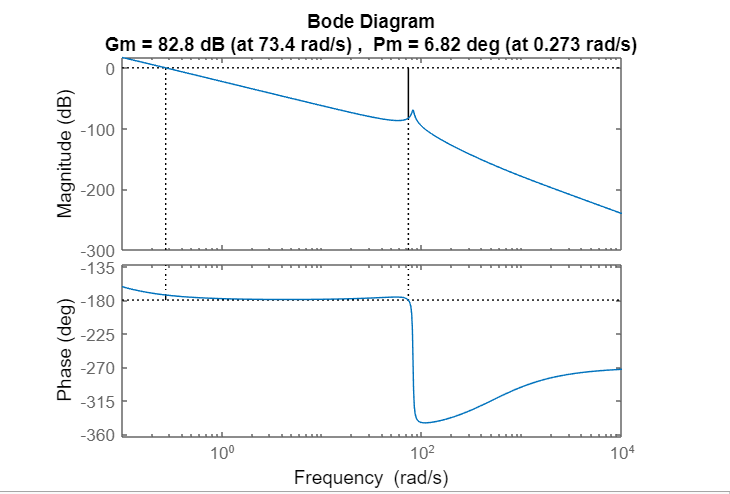
\includegraphics[width=\linewidth]{images/plot3.png}
    \label{fig:plot_3}
  \end{figure}
\end{minipage} \\[9pt]

You observe that the phase margin of the uncompensated system is way too less than what is required. \\[9pt]

\begin{minipage}{0.3\linewidth} \par
  Let us observe the root locus of the given plant.
\end{minipage}%
\hfill
\begin{minipage}{0.65\linewidth}
  \begin{figure}[H]
    \centering
    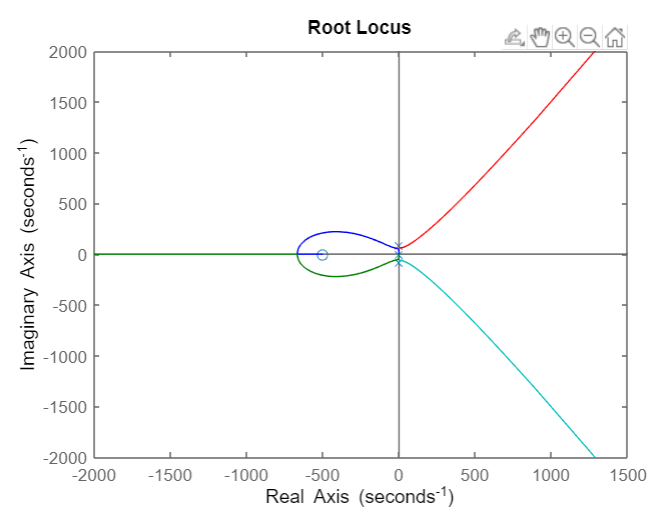
\includegraphics[width=\linewidth]{images/plot4.png}
    \label{fig:plot_4}
  \end{figure}
\end{minipage} \\[9pt]

From the root locus we can see that we need to shift the root locus to the left side and make our poles lie on the right. This is a classic example of Lead compensator. \par

Lets assume the controller is of the form,
\begin{equation}
  K_c \cdot \frac{S + Z_c}{S + P_c}
\end{equation}

The given uncompensated system,
\begin{equation}
  G(S) = \frac{S+500}{S(S+0.0325)(S^2 + 2.57S + 6667)}
\end{equation}

From the condition, \(PM = 35^\circ\). \par
Lets find the damping ratio,
\begin{equation}
  \begin{aligned}
    PM &= \tan^{-1}(\frac{2\tau}{\sqrt{-2\tau^2 + \sqrt{1 + 4\tau^4}}}) \\
    35^\circ &= \tan^{-1}(\frac{2\tau}{\sqrt{-2\tau^2 + \sqrt{1 + 4\tau^4}}}) \\
    0.7 &= \frac{2\tau}{\sqrt{-2\tau^2 + \sqrt{1 + 4\tau^4}}} \\
    \tau &= 0.316
  \end{aligned}
\end{equation}

\noindent
\subsection*{Uncompensated:}
Search along the line \(\tau = 0.316\) and \par find the operating point \(= -19.3 + 58i\) and Gain \( = 3.23 \times 10^4\) \par

\begin{figure}[H]
  \centering
  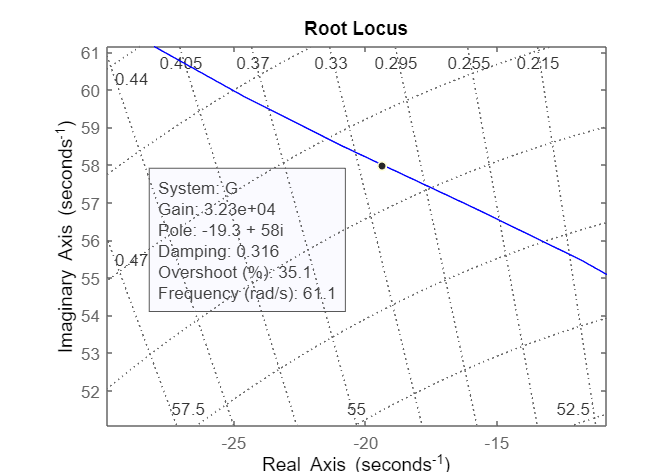
\includegraphics[width=0.8\linewidth]{images/plot5.png}
  \label{fig:plot_5}
\end{figure}

\begin{equation}
  G(S) = \frac{3.23 \times 10^4 (S+500)}{S(S+0.0325)(S^2 + 2.57S + 6667)}
\end{equation}

\begin{equation}
  \begin{aligned}
    K_v &= \lim_{S \rightarrow 0} G(S)\\
    &= \frac{32300 \times 500}{0.0325 \times 6667} = 74500
  \end{aligned}
\end{equation}

But our required value = 100. \par

\(\therefore\) The improvement of \(K_v\) from uncompensated system to compensated system,
\begin{equation}
  \frac{100}{74500} = 0.00134
\end{equation}

Our Controller \(T.f. = \frac{K(S + Z_c)}{S + P_c}\). \par

Let us arbitrarily select \(Z_c = 0.000134\), \(P_c = 0.1\) \par

Now, our \(G_c(S) = \frac{K(S + 0.000134)}{(S + 0.1)}\). \par

\begin{figure}[H]
  \centering
  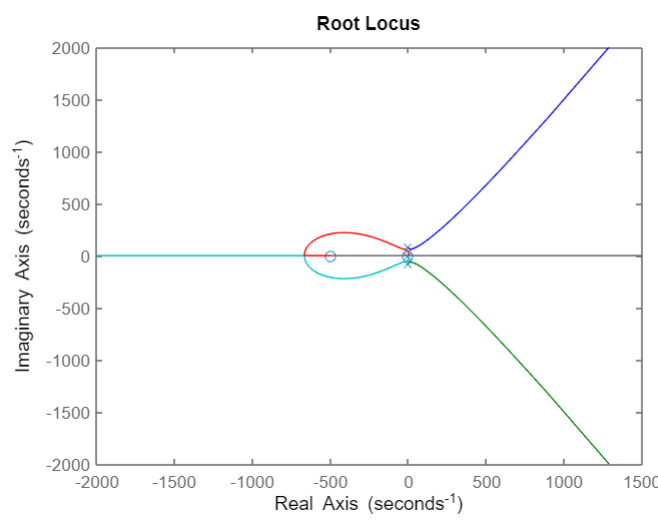
\includegraphics[width=0.8\linewidth]{images/before_plot6.png}
  \label{fig:plot_before_6}
\end{figure}

\subsection*{Compensated:}
We added a pole at -0.1 and zero at -0.000134. Search along \(\tau = 0.316\) line. \par

\begin{figure}[H]
  \centering
  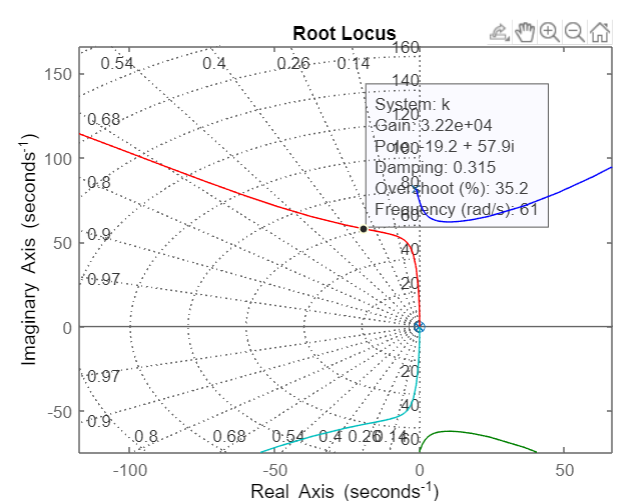
\includegraphics[width=0.8\linewidth]{images/plot6.png}
  \label{fig:plot_6}
\end{figure}

We find operating point as \(-19.2 + 57.9i\) and Gain \(= 3.22 \times 10^4\). \par

\(\therefore\) Our Final Transfer Function becomes,
\begin{equation}
  G(S) = 3.23 \times 10^4 \cdot \frac{(S+0.000134)}{(S+0.1)} \cdot \frac{(S+500)}{S(S+0.0325)(S^2 + 2.57S + 6667)}
\end{equation}

\begin{equation}
  \begin{aligned}
    K_v &= \lim_{S \rightarrow 0} G(S)\\
    &= \frac{3.22 \times 10^4 \times 0.000134 \times 500}{0.1 \times 0.0325 \times 6667} \\
    &= 99.56
  \end{aligned}
\end{equation}

\begin{figure}[H]
  \centering
  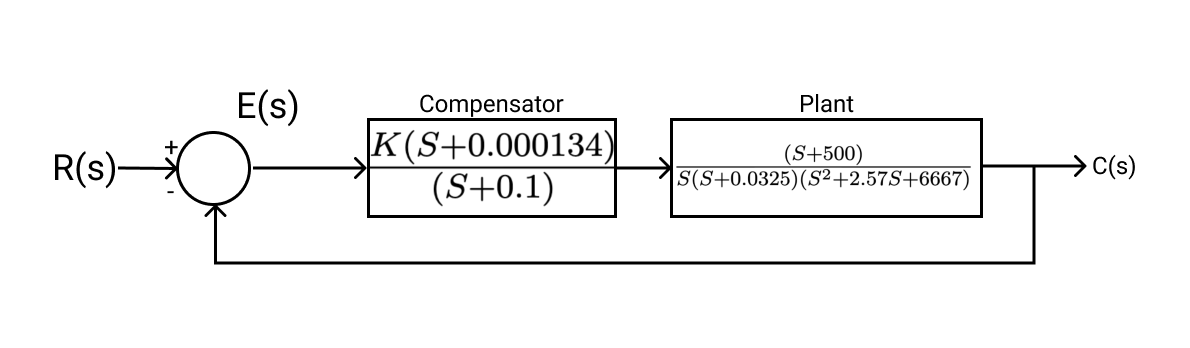
\includegraphics[width=0.8\linewidth]{images/block_diagram.png}
  \caption{Closed-loop Block Diagram}
  \label{fig:block_diagram}
\end{figure}

Let us look at the Bode diagram of the Compensated system.\par

\begin{figure}[H]
  \centering
  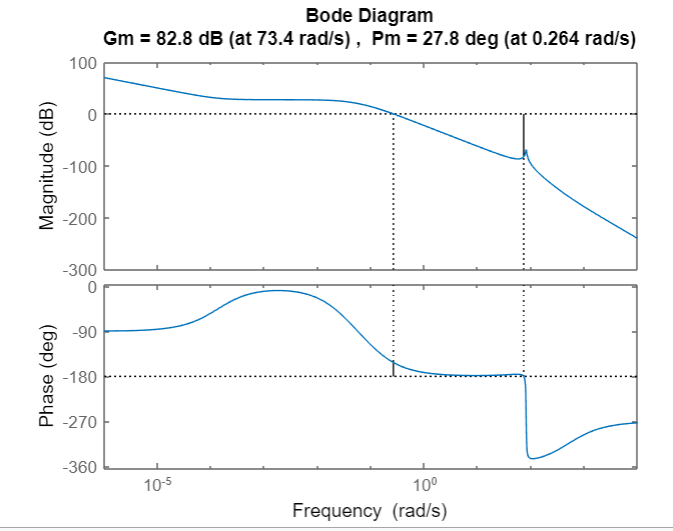
\includegraphics[width=0.8\linewidth]{images/plot7.png}
  \label{fig:plot_7}
\end{figure}

\begin{table}[H]
  \centering
  \begin{tabular}{m{0.3\linewidth}m{0.3\linewidth}m{0.4\linewidth}}
    \hline \\[2pt]
    \multicolumn{1}{>{\centering\arraybackslash}m{0.3\linewidth}}{\textbf{Parameter}} & \multicolumn{1}{>{\centering\arraybackslash}m{0.3\linewidth}}{\textbf{Uncompensated}} & \multicolumn{1}{>{\centering\arraybackslash}m{0.4\linewidth}}{\textbf{Compensated}} \\[2pt]
    \hline \\[2pt]
    Plant and Compensator & \(\frac{K(S+500)}{S(S+0.0325)(S^2 + 2.57S + 6667)}\) & \(\frac{K(S+0.000134)}{(S+0.1)}\frac{(S+500)}{S(S+0.0325)(S^2 + 2.57S + 6667)}\) \\[12pt]
    K & 32300 & 32200 \\[12pt]
    \(K_v\) & 74500 & 99.56 \\[12pt]
    Dominant Second Order Pole & \(-19.3 \pm 58i\) & \(-19.2 \pm 57.9i\) \\[6pt]
    \hline
  \end{tabular}
\end{table}

\(\therefore\) Our Controller = \(G(S) = 3.23 \times 10^4 \cdot \frac{(S+0.000134)}{(S+0.1)}\) \par with Poles = \(-19.2 + 57.9i\) \par

From above Dominant Poles,
\begin{equation}
  19.2 = \sigma = \tau \omega_n
\end{equation}
\begin{equation}
  \omega_n = 60.79\; \text{rad/s}
\end{equation}

\begin{equation}
  \begin{aligned}
    \text{Resonant Frequency} &= \omega_r = \omega_n \sqrt{1 - 2\tau^2} \\
    &= 60.79 \sqrt{1 - 2 (0.316)^2} \\
    &= 54.3\; \text{rad/s}
  \end{aligned}
\end{equation}

\begin{equation}
  \begin{aligned}
    \text{Resonant Peak} &= \frac{1}{2\tau \sqrt{1 - \tau^2}} \\
    &= \frac{1}{2 \times 0.316 \sqrt{1 - (0.316)^2}} \\
    &= 1.667
  \end{aligned}
\end{equation}

\begin{equation}
  \begin{aligned}
    \text{Bandwidth} &= \omega_n(1- 2\tau^2 + \sqrt{4\tau^4 - 4\tau^2 + 2})^{\frac{1}{2}} \\
    &= 87.69\; \text{rad/s}
  \end{aligned}
\end{equation}

Let's see both Compensated and Uncompensated transient responses.

\begin{figure}[H]
  \centering
  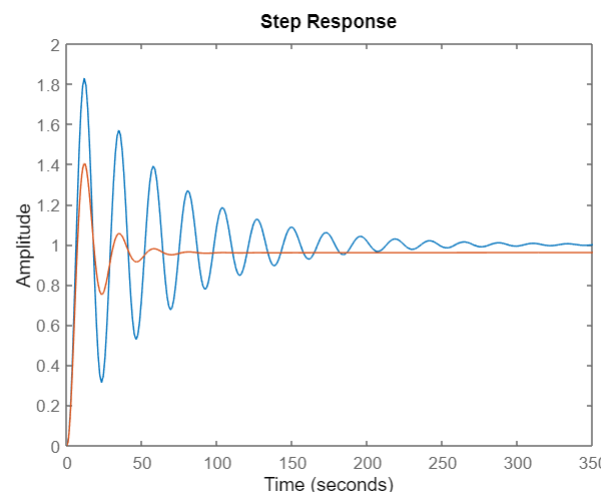
\includegraphics[width=0.8\linewidth]{images/plot8.png}
  \label{fig:plot_8}
\end{figure}

\begin{minipage}{0.45\linewidth}
  \begin{figure}[H]
    \centering
    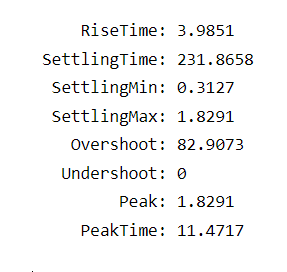
\includegraphics[width=\linewidth]{images/plot2.png}
    \label{fig:plot_2}
  \end{figure}
\end{minipage}%
\hfill
\begin{minipage}{0.45\linewidth}
  \begin{figure}[H]
    \centering
    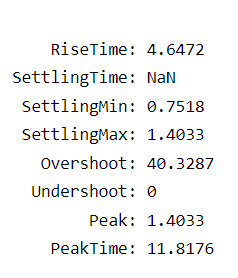
\includegraphics[width=\linewidth]{images/plot9.png}
    \label{fig:plot_9}
  \end{figure}  
\end{minipage}

\begin{minted}{matlab}
  %code for plot1
  clear all
  clc
  s = zpk(0,[],1);
  Gu =  (s+500)/(s*(s+0.0325)*(s^2+ 2.57*s+ 6667));
  stepinfo(Gu/(1+Gu))


  %code for plot2
  clear all
  clc
  s = zpk(0,[],1);
  k =  (s+500)/(s*(s+0.0325)*(s^2+ 2.57*s+ 6667));
  bode(k)


  %code for plot3
  clear all
  clc
  s = zpk(0,[],1);
  k =  (s+500)/(s*(s+0.0325)*(s^2+ 2.57*s+ 6667));
  rlocus(k)


  %Code for plot4
  clear all
  clc
  s = zpk(0,[],1);
  Gu =  (s+0.000134)(s+500)/((s+0.1)*s(s+0.0325)*(s^2+ 2.57*s+ 6667));
  rlocus(Gu)


  %code for plot5
  clear all
  clc
  s = zpk(0,[],1);
  k =  (s+0.000134)(s+500)/((s+0.1)*s(s+0.0325)*(s^2+ 2.57*s+ 6667));
  margin(k)


  %code for plot6
  clear all
  clc
  s = zpk(0,[],1);
  Gu =  (s+500)/(s*(s+0.0325)*(s^2+ 2.57*s+ 6667));

  Gc = (s+0.000134)/(s+0.1);

  Gce=Gu*Gc;
  Tu=feedback(Gu,1);
  Tc=feedback(Gce,1);
  step(Tu) 
  hold
  step(Tc)
\end{minted}

\end{document}